\setcounter{ExampleCounter}{1}
Before we can solve linear programming problems, we need to review linear equations and inequalities, because that is the language used to state optimization problems.  We'll be given a goal and the limitations on our resources in terms of linear equations and inequalities, and we'll need to graph and solve them in order to find the optimal use of our resources.

\subsection{Plotting Points}
Everything\marginnote{
\includegraphics[width=0.8\marginparwidth]{Descartes}} starts with the rectangular, or Cartesian, coordinate plane, named for Ren\'e Descartes.  As the legend goes, Descartes was lying on his bed one day, watching a fly scurry across the ceiling.  Out of idle curiosity, he wondered if there were a simple way to describe the position of the fly, and he realized that if he specified how far it was from two of the walls, that would clearly define its position.  Whether or not the legend has any basis in reality, it illustrates the idea behind the rectangular coordinate system.

\begin{center}
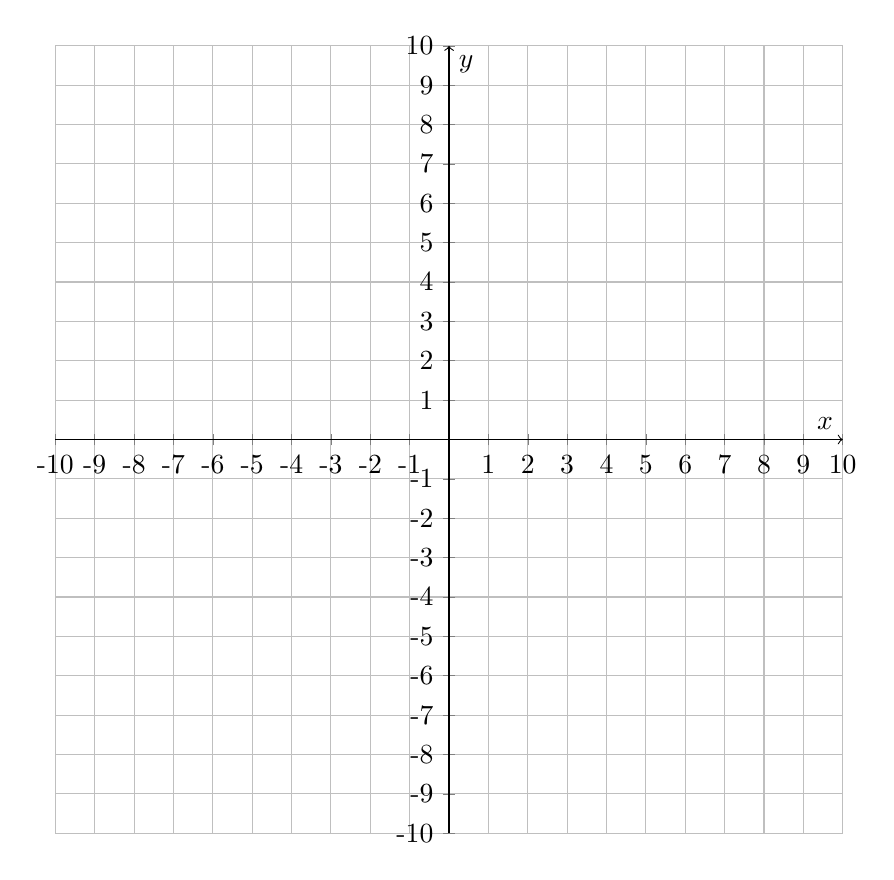
\begin{tikzpicture}
\begin{axis}[
    xmin=-10, xmax=10,
    ymin=-10, ymax=10,
    axis lines=center,
    axis on top=true,
    domain=0:1,
    x=0.5cm,
    y=0.5cm,
    xtick={-10,-9,...,10},
    xticklabels={-10,-9,...,10},
    ytick={-10,-9,...,10},
    yticklabels={-10,-9,...,10},
    axis lines=middle,
    axis line style={->},
    xlabel={$x$},
    ylabel={$y$},
    grid=major
    ]
\end{axis}
\end{tikzpicture}
\end{center}

This\marginnote{This is familiar to residents of NYC; for instance, the Metropolitan Museum of Art is located at the intersection of 5th Ave and E 82nd St} coordinate system consists of two number lines--the $x$ axis and the $y$ axis--placed at a right angle to each other, crossing at the \textbf{origin}.  You can think of the grid that these axes form as the map of a well-planned city, with north-south streets crossing east-west streets at consistent intervals.  If you want to specify a location in the city, all you have to specify is an intersection.  

This is how we plot points, by specifying their east-west location using an $x$-coordinate and specifying their north-south location using a $y$-coordinate.  These are written as an ordered pair $(x,y)$.
\pagebreak

\begin{example}[https://www.youtube.com/watch?v=5x4YS8zJ4SE]{Plotting Points}
Plot the points (0,0), (3,5), $(-2,3)$, $(-4,-4)$, and $(7,-8)$.

\sol
For each point, start at the origin and step to the right or left according to the first number in the ordered pair, then step up or down according to the second number (make sure to keep track of direction, based on whether each number is positive or negative).

\begin{center}
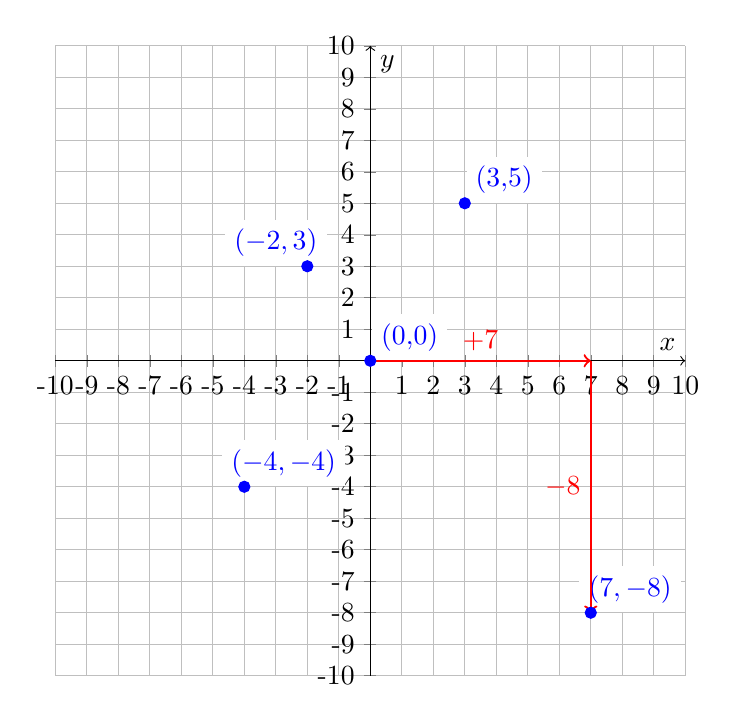
\begin{tikzpicture}
\begin{axis}[
    xmin=-10, xmax=10,
    ymin=-10, ymax=10,
    axis lines=center,
    axis on top=false,
    domain=0:1,
    x=0.4cm,
    y=0.4cm,
    xtick={-10,-9,...,10},
    xticklabels={-10,-9,...,10},
    ytick={-10,-9,...,10},
    yticklabels={-10,-9,...,10},
    axis lines=middle,
    axis line style={->},
    xlabel={$x$},
    ylabel={$y$},
    grid=major
    ]
    \addplot [only marks,color=blue] table {
	0 0
	3 5
	-2 3
	-4 -4
	7 -8
	};
	\draw [yshift=4.3cm,xshift=4.5cm] node [fill=white] {\color{blue}(0,0)};
	\draw [yshift=6.3cm,xshift=5.7cm] node [fill=white] {\color{blue}(3,5)};
	\draw [yshift=5.5cm,xshift=2.8cm] node [fill=white] {\color{blue}$(-2,3)$};
	\draw [yshift=2.7cm,xshift=2.9cm] node [fill=white] {\color{blue}$(-4,-4)$};
	\draw [yshift=1.1cm,xshift=7.3cm] node [fill=white] {\color{blue}$(7,-8)$};
	\draw [red,thick,style=->] (4 cm,4 cm) -- (6.8 cm,4 cm) node [midway,above] {\color{red} $+7$};
	\draw [red,thick,style=->] (6.8 cm,4 cm) -- (6.8 cm,0.8 cm) node [midway,left] {\color{red} $-8$};
\end{axis}
\end{tikzpicture}
\end{center}
\end{example}

\begin{try}
What points are plotted on the coordinate system shown here?
\begin{center}
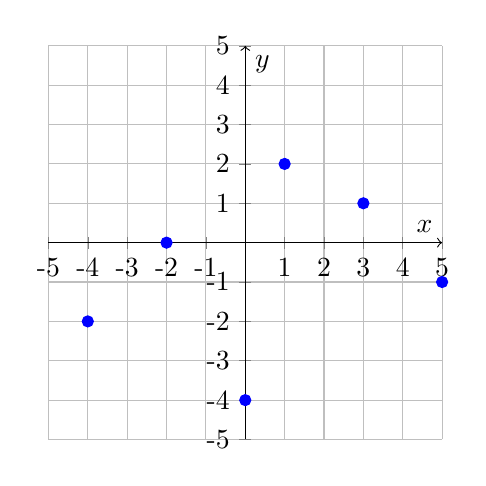
\begin{tikzpicture}
\begin{axis}[
    xmin=-5, xmax=5,
    ymin=-5, ymax=5,
    axis lines=center,
    axis on top=false,
    domain=0:1,
    x=0.5cm,
    y=0.5cm,
    xtick={-10,-9,...,10},
    xticklabels={-10,-9,...,10},
    ytick={-10,-9,...,10},
    yticklabels={-10,-9,...,10},
    axis lines=middle,
    axis line style={->},
    xlabel={$x$},
    ylabel={$y$},
    grid=major
    ]
    \addplot [only marks,color=blue] table {
	1 2
	3 1
	0 -4
	-4 -2
	5 -1
	-2 0
	};
\end{axis}
\end{tikzpicture}
\end{center}
\end{try}

Once we can plot points, we can work up from that to graphing lines (and if we wanted to, graphing all sorts of things).  Linear graphs consist of infinitely many points that all lie along a straight line that extends forever in either direction.
\vfill
\pagebreak

\subsection{Graphing Lines}
Take a look at an equation like \[y=3x+1.\]  This equation gives a relationship between $x$ and $y$; it simply says that whatever $x$ is, there is a corresponding $y$ that you get by multiplying $x$ by 3 and adding 1.  

For instance, 
\begin{center}
\begin{tabular}{l l}
if $x$ is 0, & $y$ is 1\\
if $x$ is 1, & $y$ is 4\\
if $x$ is 2, & $y$ is 7\\
if $x$ is 3, & $y$ is 10
\end{tabular}
\end{center}

We can write each of these as an ordered pair $(x,y)$, and each of those corresponds to a point on the coordinate plane:
\begin{center}
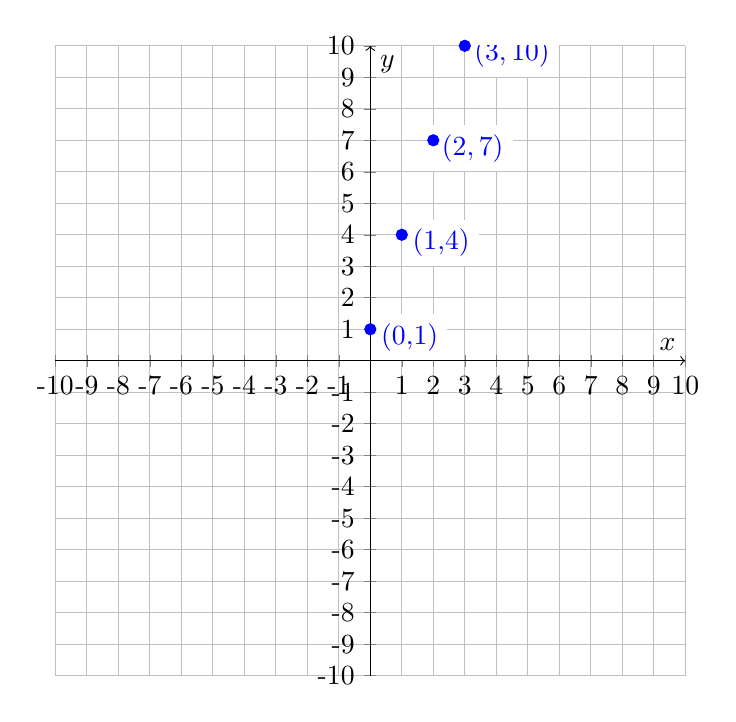
\begin{tikzpicture}
\begin{axis}[
    xmin=-10, xmax=10,
    ymin=-10, ymax=10,
    axis lines=center,
    axis on top=false,
    domain=0:1,
    x=0.4cm,
    y=0.4cm,
    xtick={-10,-9,...,10},
    xticklabels={-10,-9,...,10},
    ytick={-10,-9,...,10},
    yticklabels={-10,-9,...,10},
    axis lines=middle,
    axis line style={->},
    xlabel={$x$},
    ylabel={$y$},
    grid=major
    ]
    \addplot [only marks,color=blue] table {
	0 1
	1 4
	2 7
	3 10
	};
	\draw [yshift=4.3cm,xshift=4.5cm] node [fill=white] {\color{blue}(0,1)};
	\draw [yshift=5.5cm,xshift=4.9cm] node [fill=white] {\color{blue}(1,4)};
	\draw [yshift=6.7cm,xshift=5.3cm] node [fill=white] {\color{blue}$(2,7)$};
	\draw [yshift=7.9cm,xshift=5.8cm] node [fill=white] {\color{blue}$(3,10)$};
\end{axis}
\end{tikzpicture}
\end{center}

It's clear that all these points lie along a straight line, and if we picked $x$ values between the ones we picked, we would just be filling in the points between these.  Thus, we conclude that this is an example of a linear equation and we can draw the line that connects these dots.

\begin{center}
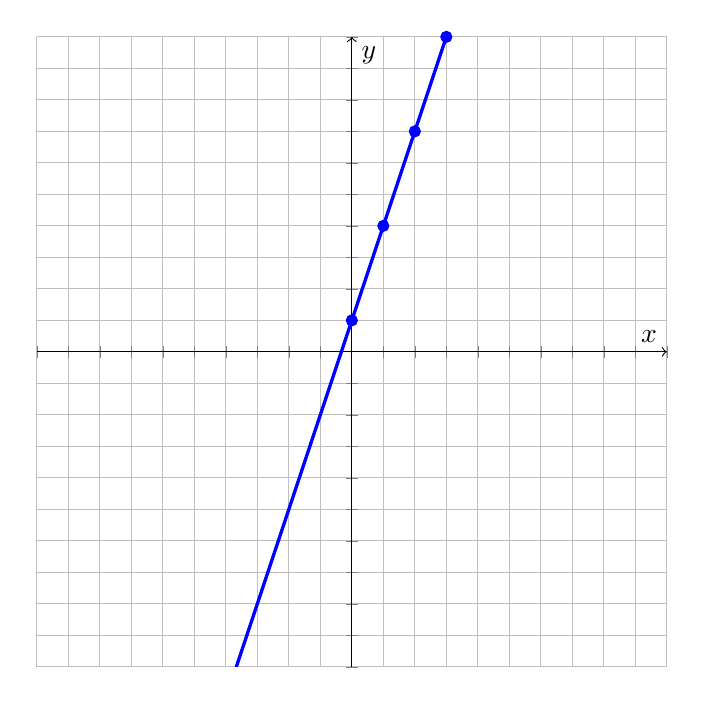
\begin{tikzpicture}
\begin{axis}[
    xmin=-10, xmax=10,
    ymin=-10, ymax=10,
    axis lines=center,
    axis on top=false,
    domain=0:1,
    x=0.4cm,
    y=0.4cm,
    xtick={-10,-9,...,10},
    xticklabels={},
    ytick={-10,-9,...,10},
    yticklabels={},
    axis lines=middle,
    axis line style={->},
    xlabel={$x$},
    ylabel={$y$},
    grid=major
    ]
    \addplot [only marks,color=blue] table {
	0 1
	1 4
	2 7
	3 10
	};
	\addplot[samples=100,domain=-10:10,very thick, blue]{3*x+1};
\end{axis}
\end{tikzpicture}
\end{center}
\vfill
\pagebreak

Notice, however, that we worked harder than we had to; once we had two points, the line was decided, and the other points just fell into place along that line.  This leads us to an important conclusion.

No matter how you graph a line, the entire process comes down to one simple fact:
\begin{formula}{Key to Graphing Lines}
\begin{center}
Two points determine a line.
\end{center}
\end{formula}
%\vspace{0.25in}
%\begin{center}
%\begin{minipage}{0.4\textwidth}
%\begin{tcolorbox}[colframe=brown!40,colback=brown!10,sharp corners=all]
%\begin{center}
%Two points determine a line
%\end{center}
%\end{tcolorbox}
%\end{minipage}
%\end{center}
%\vspace{0.25in}

Any time you graph a line, if all else fails, just try to find two points on it (by picking two sample values for $x$ like we did above and finding the corresponding $y$ values) and draw the line that passes through those two points.

\paragraph{Note} We'll only be dealing with linear equations in this chapter, but in general, you can recognize linear equations by the fact that they only have $x$'s and $y$'s and constants in them, and nothing like $x^2$ or $2^y$ or $\sqrt{x}$.  For example, each of the following are linear equations:
\begin{center}
\begin{tabular}{c}
$3x+4y=7$\\
$9x-16y=-3$\\
$y=8x-14$\\
$x=2y+5$
\end{tabular}
\end{center}
\vspace{0.5in}

\subsection{Graphing Lines Using Slope and Intercept}
Look back at that example.  The equation we started with was $y=3x+1$, and by picking a few $x$'s and plugging them into the equation to find the matching $y$'s, we got 
\begin{center}
\begin{tabular}{c c}
$x$ & $y$\\
\hline
0 & 1\\
1 & 4\\
2 & 7\\
3 & 10
\end{tabular}
\end{center}
and we could easily have kept going, or turned and starting using negative $x$ values.

However, from this table we can notice two interesting things:
\begin{enumerate}
\item Each time we increase $x$ by 1, $y$ increases by 3.  Notice that 3 is the coefficient of $x$ in the equation.  We call this the \textbf{slope}\marginnote{\small \textbf{Note:} Slope is\\ ``rise over run'': $\dfrac{\textrm{rise}}{\textrm{run}}$} of the equation, because it describes how the line is angled.  Look back at the graph and notice how, traveling from left to right, the line travels upward 3 units for every unit forward.
\item When $x$ is 0, $y$ is 1, which is the constant in the equation (this is not accidental).  This is called the \textbf{$y$-intercept}, because it is the point where the line crosses the $y$-axis.  Look back at the graph and notice how the line crosses the $y$-axis at 1.
\end{enumerate}

This gives us a quick way to graph a line that is written in \textit{slope-intercept form}: $y=mx+b$, where $m$ is the slope and $b$ is the $y$-intercept.  It's still based on graphing by plotting two points: we can graph the intercept first, then go right one unit and up or down however many units the slope tells us to and plot a second point, then connect these two dots.
\vfill
\pagebreak

\begin{example}[https://www.youtube.com/watch?v=Xh3O0YEgwnM]{Graphing Using Slope and Intercept}
Graph the line $y=-2x+4$.

\sol
In this equation, the slope is $-2$ and the intercept is 4.  We know then that the line crosses the $y$-axis at 4 and travels down two units for every one it travels to the right:
\begin{center}
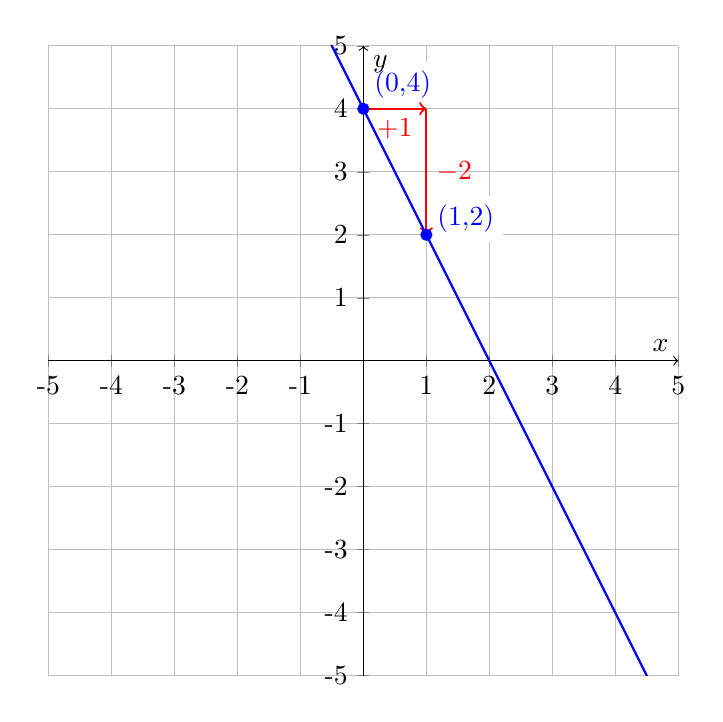
\begin{tikzpicture}
\begin{axis}[
    xmin=-5, xmax=5,
    ymin=-5, ymax=5,
    axis lines=center,
    axis on top=false,
    domain=0:1,
    x=0.8cm,
    y=0.8cm,
    xtick={-10,-9,...,10},
    xticklabels={-10,-9,...,10},
    ytick={-10,-9,...,10},
    yticklabels={-10,-9,...,10},
    axis lines=middle,
    axis line style={->},
    xlabel={$x$},
    ylabel={$y$},
    grid=major
    ]
    \addplot [only marks,color=blue] table {
	0 4
	1 2
	};
	\draw [yshift=8.3cm,xshift=4.5cm] node [fill=white] {\color{blue}(0,4)};
	\draw [yshift=6.6cm,xshift=5.3cm] node [fill=white] {\color{blue}(1,2)};
	\draw [red,thick,style=->] (4 cm,8 cm) -- (4.8 cm,8 cm) node [midway,below] {\color{red} $+1$};
	\draw [red,thick,style=->] (4.8 cm,8 cm) -- (4.8 cm,6.4 cm) node [midway,right] {\color{red} $-2$};
	\addplot[samples=100,domain=-5:5,thick,blue]{-2*x+4};
\end{axis}
\end{tikzpicture}
\end{center}
\end{example}

\begin{try}[http://hartleymath.com/versatilemath/tryit/\#/linear-programming--find-equation-of-line-graphed]
Find the equation of the line graphed below in slope-intercept form.
\begin{center}
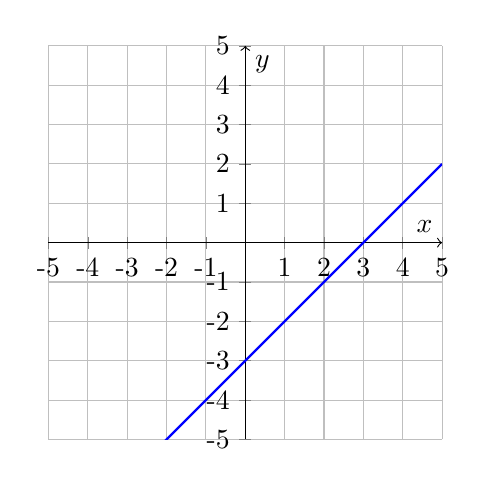
\begin{tikzpicture}
\begin{axis}[
    xmin=-5, xmax=5,
    ymin=-5, ymax=5,
    axis lines=center,
    axis on top=false,
    domain=0:1,
    x=0.5cm,
    y=0.5cm,
    xtick={-10,-9,...,10},
    xticklabels={-10,-9,...,10},
    ytick={-10,-9,...,10},
    yticklabels={-10,-9,...,10},
    axis lines=middle,
    axis line style={->},
    xlabel={$x$},
    ylabel={$y$},
    grid=major
    ]
    
	\addplot[samples=100,domain=-5:5,thick,blue]{x-3};
\end{axis}
\end{tikzpicture}
\end{center}
\end{try}

Of course, if a linear equation is not written in slope intercept form, a little algebra can manipulate it until it is:
\begin{align*}
4x+2y &= 8\\
2y &= -4x +8\\
y &= -2x+4
\end{align*}

\begin{proc}{Using Your Calculator}
You can also use a graphing calculator to graph a linear equation if it is written in slope-intercept form.  To do so, press the Y= button in the upper lefthand corner and enter the equation, using the $X,T,\theta,n$ button to enter $x$.  Then press GRAPH to see the line.
\begin{center}
\begin{tabular}{c c}
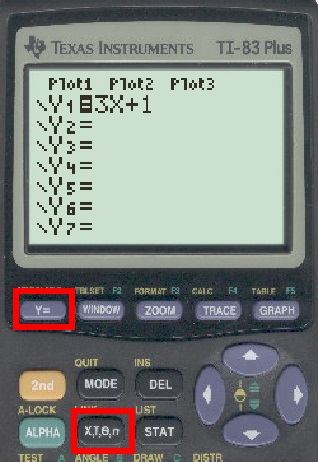
\includegraphics[height=2in]{CalcLine1} & \hspace{0.5in} 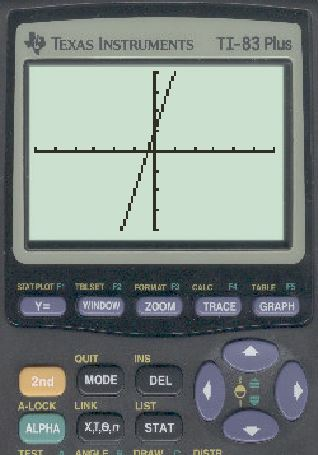
\includegraphics[height=2in]{CalcLine2}
\end{tabular}
\end{center}
\end{proc}

\subsection{Graphing Lines Using Intercepts}
Remember, whenever we graph a line, we're relying on the principle that \textbf{\emph{two points determine a line}}.
%\begin{center}
%\begin{minipage}{0.5\textwidth}
%\begin{tcolorbox}[colframe=brown!40,colback=brown!10,sharp corners=all]
%\begin{center}
%Two points determine a line.
%\end{center}
%\end{tcolorbox}
%\end{minipage}
%\end{center}

Any two points that lie on the line will do; however, in the examples we'll be doing in this chapter, it will often simplify things if we use a specific set of two points, namely the \textbf{intercepts}.

We've already seen the $y$-intercept, the point where the line crosses the $y$-axis.  The $x$-intercept, naturally, is the point where the line crosses the $x$-axis.
\begin{center}
\begin{tikzpicture}
\begin{axis}[
    xmin=-7, xmax=7,
    ymin=-5, ymax=5,
    axis lines=center,
    axis on top=false,
    domain=0:1,
    x=0.8cm,
    y=0.8cm,
    xtick={},
    xticklabels={},
    ytick={},
    yticklabels={},
    axis lines=middle,
    axis line style={->},
    xlabel={$x$},
    ylabel={$y$},
    %grid=major
    ]
    \addplot [only marks,color=blue] table {
	0 3
	3 0
	};
	\draw [yshift=4.5cm,xshift=9.5cm] node [fill=white] {\large\color{blue} $x$-intercept: ($a$,0)};
	\draw [yshift=6.8cm,xshift=7.5cm] node [fill=white] {\large\color{blue} $y$-intercept: (0,$b$)};
	\addplot[samples=100,domain=-5:7,thick,blue]{3-x};
\end{axis}
\end{tikzpicture}
\end{center}
\pagebreak

Notice the key point about intercepts (this is how we'll find them): 
\begin{itemize}
\item At the $x$-intercept, the $y$-coordinate is always 0
\item At the $y$-intercept, the $x$-coordinate is always 0
\end{itemize}

Thus, finding the intercepts will come down to filling in the missing pieces in the following table:
\begin{center}
{\Large
\begin{tabular}{c | c}
$x$ & $y$\\
\hline
0 & \\
 & 0\\
\end{tabular}}
\end{center}

\begin{example}[https://www.youtube.com/watch?v=n5OfmqNGLmI]{Graphing Lines Using Intercepts}
Graph the line $x-0.5y=5$ using the intercepts.

\sol
\begin{itemize}
\item Find the $x$-intercept: let $y=0$ and find its corresponding $x$ value:
\[x-0.5(0)=5 \longrightarrow x=5\]
\item Find the $y$-intercept: let $x=0$ and find its corresponding $y$ value:
\[0-0.5y=5 \longrightarrow -0.5y=5 \longrightarrow y=\dfrac{5}{-0.5}=-10\]
\end{itemize}

The intercepts are thus $(5,0)$ and $(0,-10)$, and we can graph the line by plotting these two points and connecting them.
\begin{center}
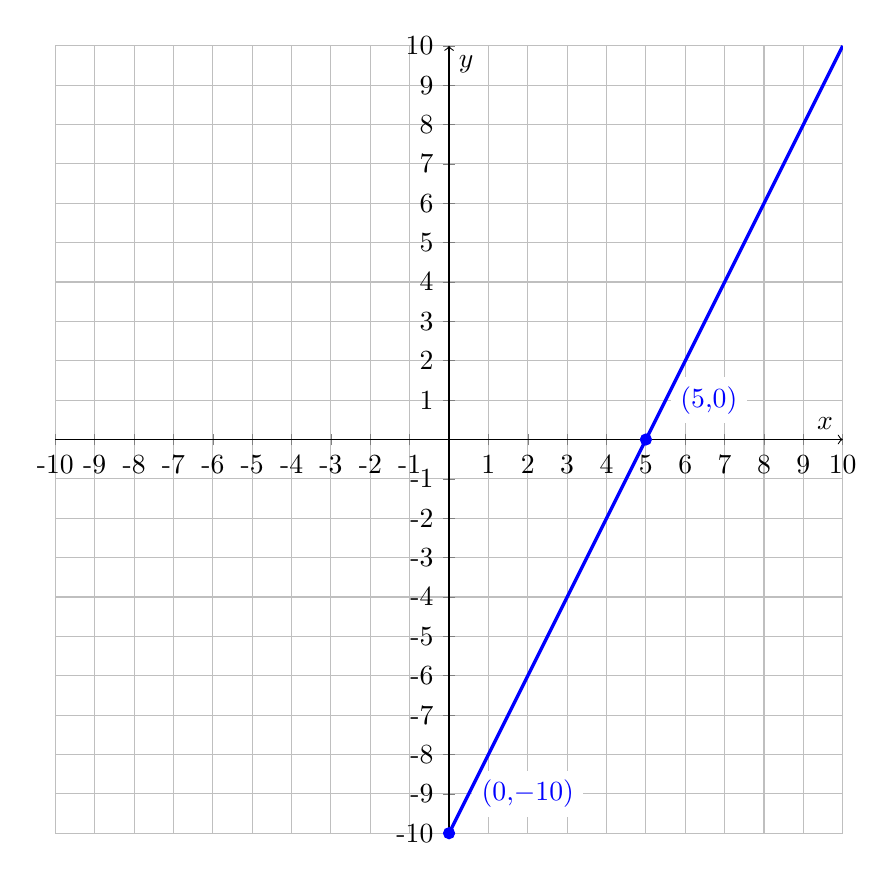
\begin{tikzpicture}
\begin{axis}[
    xmin=-10, xmax=10,
    ymin=-10, ymax=10,
    axis lines=center,
    axis on top=false,
    domain=0:1,
    x=0.5cm,
    y=0.5cm,
    xtick={-10,-9,...,10},
    xticklabels={-10,-9,...,10},
    ytick={-10,-9,...,10},
    yticklabels={-10,-9,...,10},
    axis lines=middle,
    axis line style={->},
    xlabel={$x$},
    ylabel={$y$},
    grid=major
    ]
    \addplot [only marks,color=blue] table {
	0 -10
	5 0
	};
	\draw [yshift=10.5cm,xshift=6cm] node [fill=white] {\color{blue} (0,$-10$)};
	\draw [yshift=15.5cm,xshift=8.3cm] node [fill=white] {\color{blue} (5,0)};
	\addplot[samples=100,domain=-10:10,very thick,blue]{2*x-10};
\end{axis}
\end{tikzpicture}
\end{center}
\end{example}
\pagebreak

\begin{example}[https://www.youtube.com/watch?v=SkjLSvZBe0g]{Graphing Lines Using Intercepts}
Graph the line $2x+y=8$ using the intercepts.

\sol
\begin{itemize}
\item Find the $x$-intercept: let $y=0$ and find its corresponding $x$ value:
\[2x+(0)=8 \longrightarrow x=\dfrac{8}{2}=4\]
\item Find the $y$-intercept: let $x=0$ and find its corresponding $y$ value:
\[2(0)+y=8 \longrightarrow y=8\]
\end{itemize}

The intercepts are thus $(4,0)$ and $(0,8)$, and we can graph the line by plotting these two points and connecting them.
\begin{center}
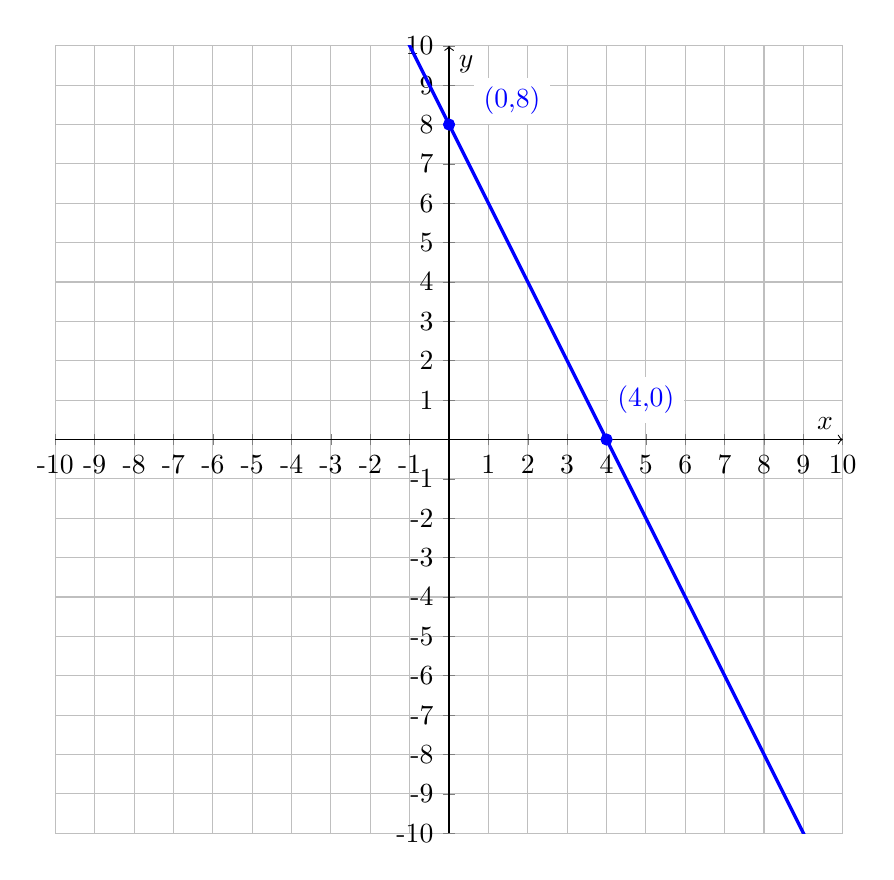
\begin{tikzpicture}
\begin{axis}[
    xmin=-10, xmax=10,
    ymin=-10, ymax=10,
    axis lines=center,
    axis on top=false,
    domain=0:1,
    x=0.5cm,
    y=0.5cm,
    xtick={-10,-9,...,10},
    xticklabels={-10,-9,...,10},
    ytick={-10,-9,...,10},
    yticklabels={-10,-9,...,10},
    axis lines=middle,
    axis line style={->},
    xlabel={$x$},
    ylabel={$y$},
    grid=major
    ]
    \addplot [only marks,color=blue] table {
	0 8
	4 0
	};
	\draw [yshift=10.3cm,xshift=5.8cm] node [fill=white] {\color{blue} (0,8)};
	\draw [yshift=6.5cm,xshift=7.5cm] node [fill=white] {\color{blue} (4,0)};
	\addplot[samples=100,domain=-10:10,very thick,blue]{-2*x+8};
\end{axis}
\end{tikzpicture}
\end{center}
\end{example}
\vfill
\pagebreak

\subsection{Horizontal and Vertical Lines}
Lastly, we will need to be able to easily recognize and graph horizontal and vertical lines.  Think for a moment for what it means for a line to be horizontal: for every $x$ value, the $y$ value of a point on the line is the same constant.  Thus, whenever we see an equation that looks like \[y=b\] for any constant $b$, we'll know that it is a horizontal line at $b$.  Similarly, on a vertical line, the $x$-coordinate is consistent for any $y$ value, so vertical lines have the form \[x=a\] for some constant $a$.

\begin{example}[https://www.youtube.com/watch?v=zL75FqUbJAk]{Graphing Horizontal and Vertical Lines}
Graph the lines $y=3$ and $x=-2$.\\

\sol
The line $y=3$ is a horizontal one at 3, and $x=-2$ is a vertical line at $-2$:
\begin{center}
\begin{tikzpicture}
\begin{axis}[
    xmin=-5, xmax=5,
    ymin=-5, ymax=5,
    axis lines=center,
    axis on top=false,
    domain=0:1,
    x=0.8cm,
    y=0.8cm,
    xtick={-10,-9,...,10},
    xticklabels={-10,-9,...,10},
    ytick={-10,-9,...,10},
    yticklabels={-10,-9,...,10},
    axis lines=middle,
    axis line style={->},
    xlabel={$x$},
    ylabel={$y$},
    %grid=major
    ]
    \addplot [red,ultra thick] coordinates{(-2,-5)(-2,5)};
    \addplot [blue,ultra thick] coordinates{(-5,3)(5,3)};
    \node (A) at (axis cs:-3,1.5) {\large\color{red} $x=-2$};
    \node (B) at (axis cs:2.5,3.5) {\large\color{blue} $y=3$};
\end{axis}
\end{tikzpicture}
\end{center}
\end{example}

\begin{proc}{Summary: Horizontal and Vertical Lines}
\begin{itemize}
\item Horizontal lines have the form \[y=b.\]
\item Vertical lines have the form \[x=a.\]
\end{itemize}
\end{proc}